\documentclass[conference, 11pt]{IEEEtran}
\IEEEoverridecommandlockouts
% The preceding line is only needed to identify funding in the first footnote. If that is unneeded, please comment it out.
\usepackage{cite}
\usepackage{amsmath,amssymb,amsfonts}
\usepackage{algorithmic}
\usepackage{graphicx}
\usepackage{textcomp}
\usepackage{xcolor}
\usepackage{hyperref}
\hypersetup{
colorlinks=true,
linkcolor=blue,
filecolor=blue,
citecolor=black,      
urlcolor=cyan,
}
\def\BibTeX{{\rm B\kern-.05em{\sc i\kern-.025em b}\kern-.08em
    T\kern-.1667em\lower.7ex\hbox{E}\kern-.125emX}}
\begin{document}

\bstctlcite{IEEEexample:BSTcontrol}

\makeatletter
\newcommand{\linebreakand}{%
  \end{@IEEEauthorhalign}
  \hfill\mbox{}\par
  \mbox{}\hfill\begin{@IEEEauthorhalign}
}
\makeatother

\title{SAIRA: Student Affairs AI Response Assistant}

\author{\IEEEauthorblockN{Vladimir Makharev}
\IEEEauthorblockA{\textit{Innopolis University}\\
Innopolis, Russia \\
\href{mailto:v.makharev@innopolis.university}{v.makharev@innopolis.university}}
\and
\IEEEauthorblockN{Artem Batalov}
\IEEEauthorblockA{\textit{Innopolis University}\\
Innopolis, Russia \\
\href{a.batalov@innopolis.university}{a.batalov@innopolis.university}}
\linebreakand
\IEEEauthorblockN{Danil Andreev}
\IEEEauthorblockA{\textit{Innopolis University}\\
Innopolis, Russia \\
\href{d.andreev@innopolis.university}{d.andreev@innopolis.university}}
\and
\IEEEauthorblockN{Evgenii Evlampev}
\IEEEauthorblockA{\textit{Innopolis University}\\
Innopolis, Russia \\
\href{e.evlampev@innopolis.university}{e.evlampev@innopolis.university}}
}

\maketitle

\begin{abstract}
Lorem Ipsum dolor TODO ... 
GitHub link to the project: \href{https://github.com/kilimanj4r0/SAIRA}{https://github.com/kilimanj4r0/SAIRA}
\end{abstract}

\begin{IEEEkeywords}
LLM, knowledge base, chat-bot
\end{IEEEkeywords}

\section{Introduction}

\begin{figure}[h]
\centering

\includegraphics[width=0.4\linewidth]{saira.png}
\caption{Project Logo}
\end{figure}

Through the years, knowledge base systems have been developed to support many organizational processes. One of the most transformational applications has been AI-powered customer support, including self-service options.

Innopolis University has the \href{http://omnidesk.ru}{omnidesk.ru} support system for students. The system is a customer support platform designed to streamline and enhance customer service interactions. However, this system is not capable of automatically answering trivial requests from students.

According to Student Affairs Office, approximately $20\%$ of all requests to the system is trivial and can be answered automatically, based on University knowledge base.

\section{Related work}
The Transformer Architecture \cite{attention_is_all_you_need} has improved the state-of-the-art in various sequence modeling tasks. Transformer-based Large Language Models (LLM), such as GPT \cite{gpt}, LLaMA \cite{llama}, and Mistral \cite{mistral}, with billions of parameters, have displayed near-human or sometimes even superhuman performance on specific tasks. The capability to process and generate coherent and contextually relevant text has led to their widespread adoption.

One of the possible applications of LLMs is as domain-specific knowledge base assistants, where models excel in providing tailored information and insights across various specialized fields. In this role, LLMs can interpret and respond to intricate queries in a conversational manner, making them particularly useful as support assistants. Nevertheless, their proficiency in accessing and meticulously managing knowledge is somewhat restricted. Therefore, in tasks that demand substantial knowledge, their effectiveness is not as advanced as task-specific systems. Furthermore, the challenges of tracing the origins of their decisions and keeping their global knowledge up-to-date are still areas of ongoing research.

\subsection{Fine-tuning LLM}
Fine-tuning adapts the LLM's weights to custom domains and tasks.

Data scientists feed the model a collection of prompts and expected responses. The model learns the gaps between what it currently produces and what the training pipeline expected and adjusts its \emph{attention} to specific features and patterns.

However, fine-tuning requires a large amount of labeled data, which may be scarce, noisy, or expensive to obtain. It also requires significant computational resources, which could present a significant hurdle, so it is difficult to fine-tune new model regularly on new data.

\subsection{Retrieval Augmented Generation (RAG)}

\begin{figure}[h]
\centering
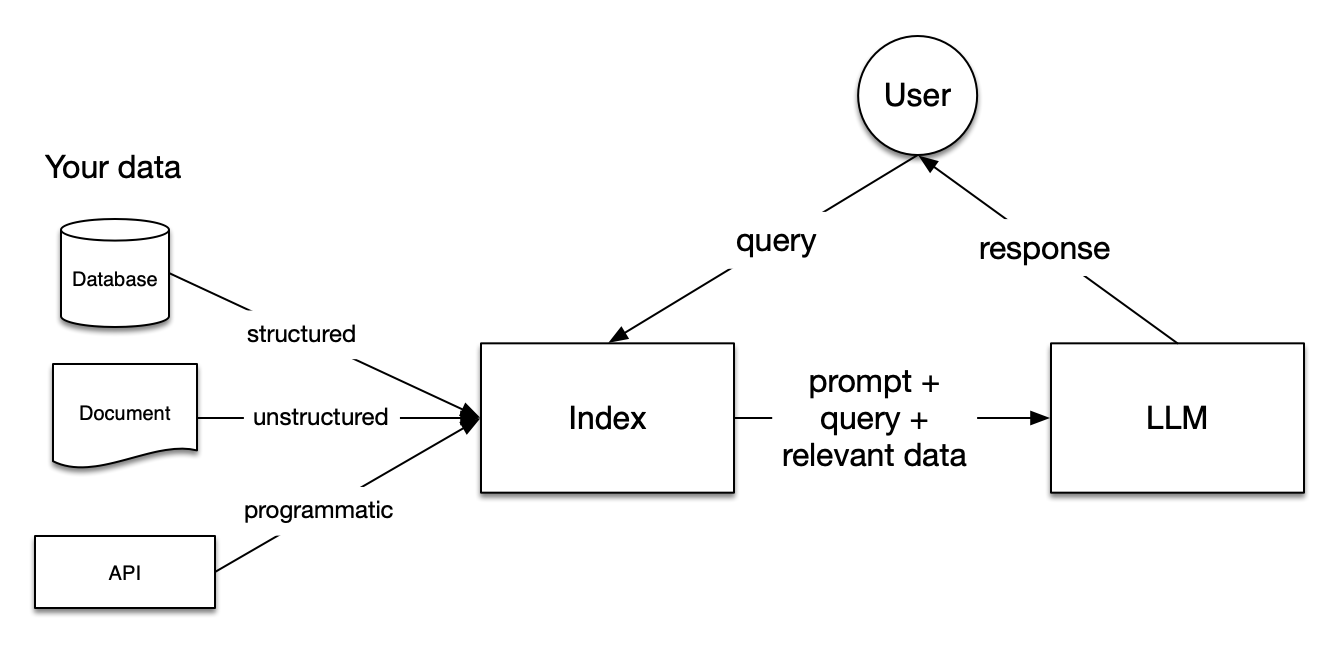
\includegraphics[width=1.0\linewidth]{basic_rag.png}
\caption{Overview of RAG approach \cite{llamaindex_rag}}
\end{figure}

Retrieval Augmented Generation (RAG) \cite{rag} inserts an additional step between users' requests and the generative model. In this step, the pipeline finds information relevant to the user's request and injects it as context. The data is loaded and prepared for queries or ``indexed''. User queries act on the index, which filters your data down to the most relevant context. This context and your query then go to the LLM along with a prompt, and the LLM provides a response. This information could come from:
\begin{itemize}
    \item A vector database such as FAISS \cite{faiss} or Pinecone;
    \item Unstructured documents;
    \item Traditional databases such as SQL or MongoDB;
    \item APIs such as those for Google Maps or IMDB;
    \item A search engine such as Google or Bing.
\end{itemize}

As stated in \cite{rag}, human evaluators were provided with a topic and given two questions in the style of Jeopardy that the topic would respond to. The system inquired which question they deemed more based on facts. Comparatively, the responses from the model improved with RAG were judged as factual $54.4\%$ of the time, in contrast to only $18.8\%$ for the model without RAG enhancement.


\section{Methodology}

\subsection{Information Retrieval}

We have aggregated a catalog of university websites speculated to encompass valuable information. For detailed listings, please consult Table \ref{tab:university_websites}, which outlines these relevant sources.

The data from websites is gathered through parsers. Utilizing parsers enables the automation of data collection, updates, and formatting, significantly contributing to the accuracy of responses generated by Large Language Model (LLM). All parsers are scripted in Python and employ auxiliary packages to extract and format primary information from the websites.

Due to the disparate formats in which information is presented across various websites, distinct packages were employed for different sites. For parsing \href{https://eduwiki.innopolis.university/}{eduwiki.innopolis.university} and \href{https://campuslife.innopolis.ru/}{campuslife.innopolis.ru}, the \texttt{markdownify} package was utilized to convert HTML pages into markdown format. Additionally, \textit{readability} was used for \href{https://campuslife.innopolis.ru/}{campuslife.innopolis.ru} to extract key information from the page, given its abundance of navigational elements and news posts.

\begin{table*}[h] % Use t, b, or h as per your preference for table positioning
\caption{List of University Websites with Data}
\centering
\begin{tabular}{|l|l|l|}
\hline
\textbf{Website} & \textbf{Data} & \textbf{Link} \\
\hline
University & General Information & \url{https://innopolis.university/} \\
EduWiki & Information on educational programs & \url{https://eduwiki.innopolis.university/} \\
Campus & Information about campus life & \url{https://campuslife.innopolis.ru/} \\
Hotel & Support for accommodation-related queries & \url{https://hotel.innopolis.university/} \\
Sport & Sports for students & \url{https://sport.innopolis.university/} \\
InnoHassle & Schedules & \url{https://innohassle.ru/schedule} \\
\hline
\end{tabular}
\label{tab:university_websites}
\end{table*}


\subsection{RAG + LlamaIndex}
There are five key stages within RAG.
\subsubsection{Loading stage}
The loading is getting the data from retrieved files. 

We use \texttt{SimpleDirectoryReader} for loading all our data to the pipeline in a LlamaIndex's \texttt{Document} container, then using \texttt{Node} to represent a ``chunk'' of a source \texttt{Document}.

\subsubsection{Indexing stage}
The indexing is creating a data structure that allows for querying the data. For LLMs this often means creating vector embeddings.

\begin{figure}[h]
\centering
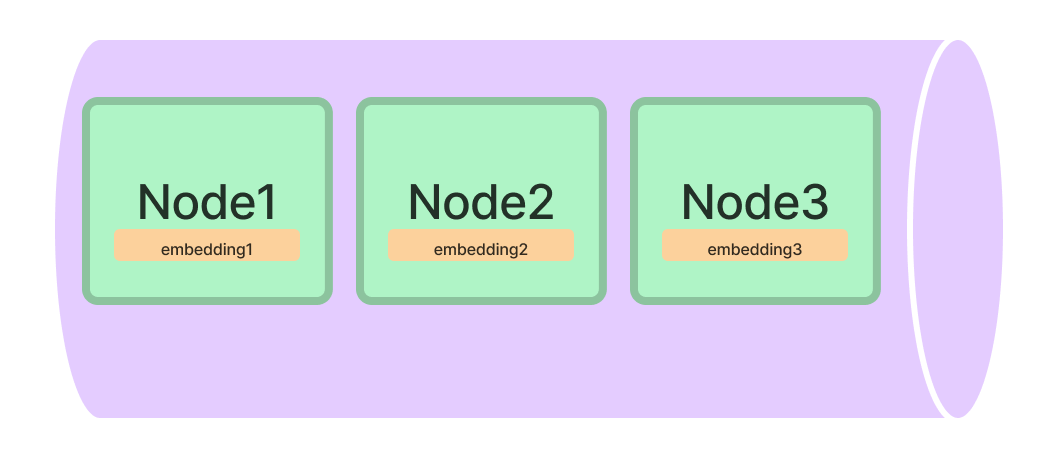
\includegraphics[width=0.8\linewidth]{vector_store.png}
\caption{Vector Store index}
\label{fig:vector_store}
\end{figure}

For our system we use Vector Store index (Fig. \ref{fig:vector_store}). This type index stores each Node and a corresponding embedding.

\subsubsection{Storing stage}

\begin{itemize}
    \item \textbf{Loading:} getting your data from somewhere - whether it's text files, PDFs, another website, a database, or an API - into your pipeline;
    \item \textbf{Indexing:} creating a data structure that allows for querying the data. For LLMs this often means creating vector embeddings;
    \item \textbf{Querying:} utilize LLMs and LlamaIndex data structures to query, including sub-queries, multi-step queries and hybrid strategies;
    \item \textbf{Evaluation:} measures of how accurate, faithful and fast your responses to queries are.
\end{itemize}

% TODO

\section{Experiments}

% TODO

\section{Evaluation}

% TODO

\section{Analysis}

% TODO

\section{Conclusion}

% TODO

\section{Future Work}

As we continue to enhance the capabilities of our AI assistant tailored for answering student queries, several avenues for future development have been identified. One significant expansion involves the incorporation of (scanned) document parsing, enabling the system to extract information from various document formats to enrich its knowledge base. Additionally, accommodating both English and Russian documents, particularly in scenarios where questions and answers are in English within Russian documents, poses an interesting challenge. This could potentially involve leveraging multilingual models or integrating translation mechanisms within the pipeline to ensure seamless comprehension and response generation. These proposed enhancements aim to broaden the AI assistant's scope and improve its efficiency in handling diverse linguistic and informational contexts, thereby augmenting its utility for our users.

% --------------------------------------------------------------------

\bibliographystyle{IEEEtran}
\bibliography{references}
\end{document}
